\documentclass[10pt,oneside]{article}
\usepackage[T1]{fontenc}
\usepackage[utf8]{inputenc}
%\usepackage[latin1]{inputenc}
\DeclareUnicodeCharacter{00A0}{ }
% \usepackage{lmodern}
%\usepackage[adobe-utopia,uppercase=upright,greeklowercase=upright]{mathdesign}
\usepackage[adobe-utopia]{mathdesign}
%\usepackage{minionpro}
% \usepackage{pifont}
% \usepackage{amssymb}
\usepackage{amsmath}
\usepackage[francais]{babel}
% \usepackage[francais]{varioref}
\usepackage[dvips]{graphicx}
\usepackage{here}
\usepackage{framed}
\usepackage[normalem]{ulem}
\usepackage{fancyhdr}
\usepackage{titlesec}
\usepackage{vmargin}
\usepackage{longtable}

\usepackage{amsmath}

\usepackage{ifthen}
%\usepackage[•]{caption}

%\usepackage{epsfig}
\usepackage{subfig}

\usepackage{multirow}
\usepackage{multicol} % Portions de texte en colonnes
\usepackage{flafter}%floatants après la référence



\usepackage{color}
\usepackage{colortbl}


\definecolor{gris25}{gray}{0.75}
\definecolor{bleu}{RGB}{18,33,98}
\definecolor{bleuf}{RGB}{42,94,171}
\definecolor{bleuc}{RGB}{231,239,247}
\definecolor{rougef}{RGB}{185,18,27}
\definecolor{rougec}{RGB}{255,230,231}
\definecolor{vertf}{RGB}{103,126,82}
\definecolor{vertc}{RGB}{220,255,191}
\definecolor{violetf}{RGB}{112,48,160}
\definecolor{violetc}{RGB}{230,224,236}
\definecolor{jaunec}{RGB}{220,255,191}


\newenvironment{corrige}[1][\hsize]%
{%
    \def\FrameCommand
    {%
\rotatebox{90}{\textit{\textsf{Correction}}} 
        {\color{violetf}\vrule width 3pt}%
        \hspace{0pt}%must no space.
        \fboxsep=\FrameSep\colorbox{violetc}%
    }%
    \MakeFramed{\hsize#1\advance\hsize-\width\FrameRestore}%
}%
{\endMakeFramed}%



\newenvironment{sci}[1][\hsize]%
{%
    \def\FrameCommand%
    {%
%\rotatebox{90}{\textit{\textsf{Scilab}}
\includegraphics[height=.8cm]{png/logo_scilab}} 
\rotatebox{90}{
\includegraphics[height=.6cm]{png/logo_scilab}} 
        {\color{violetf}\vrule width 3pt}%
        \hspace{0pt}%must no space.
        \fboxsep=\FrameSep\colorbox{violetc}%
    }%
    \MakeFramed{\hsize #1 \advance\hsize-\width\FrameRestore}%
}%
{\endMakeFramed}%

\newenvironment{pseudo}[1][\hsize]%
{%
    \def\FrameCommand%
    {%
\rotatebox{90}{\textit{\textsf{Pseudo Code}}} 
        {\color{violetf}\vrule width 3pt}%
        \hspace{0pt}%must no space.
        \fboxsep=\FrameSep\colorbox{violetc}%
    }%
    \MakeFramed{\hsize #1 \advance\hsize-\width\FrameRestore}%
}%
{\endMakeFramed}%

\newenvironment{py}[1][\hsize]%
{%prof
    \def\FrameCommand%
    {%
%\rotatebox{90}{\textit{\textsf{Python}}} 
\rotatebox{90}{
\includegraphics[height=.6cm]{png/logo_python}} 
        {\color{violetf}\vrule width 3pt}%
        \hspace{0pt}%must no space.
        \fboxsep=\FrameSep\colorbox{violetc}%
    }%
    \MakeFramed{\hsize #1 \advance\hsize-\width\FrameRestore}%
}%
{\endMakeFramed}%


\newenvironment{term}[1][\hsize]%
{%
    \def\FrameCommand%
    {%
\rotatebox{90}{\textit{\textsf{Terminal}}} 
        {\color{violetf}\vrule width 3pt}%
        \hspace{0pt}%must no space.
        \fboxsep=\FrameSep\colorbox{violetc}%
    }%
    \MakeFramed{\hsize #1 \advance\hsize-\width\FrameRestore}%
}%
{\endMakeFramed}%


\newenvironment{rem}[1][\hsize]%
{%
    \def\FrameCommand
    {%
\rotatebox{90}{\textit{\textsf{Remarque}}} 
        {\color{bleuf}\vrule width 3pt}%
        \hspace{0pt}%must no space.
        \fboxsep=\FrameSep\colorbox{bleuc}%
    }%
    \MakeFramed{\hsize#1\advance\hsize-\width\FrameRestore}%
}%
{\endMakeFramed}%


\newenvironment{savoir}[1][\hsize]%
{%
    \def\FrameCommand
    {%
\rotatebox{90}{\textit{\textsf{Savoir}}} 
        {\color{bleuf}\vrule width 3pt}%
        \hspace{0pt}%must no space.
        \fboxsep=\FrameSep\colorbox{bleuc}%
    }%
    \MakeFramed{\hsize#1\advance\hsize-\width\FrameRestore}%
}%
{\endMakeFramed}%

\newenvironment{Objectif}[1][\hsize]%
{%
    \def\FrameCommand
    {%
\rotatebox{90}{\textit{\textsf{Objectif}}} 
        {\color{bleuf}\vrule width 3pt}%
        \hspace{0pt}%must no space.
        \fboxsep=\FrameSep\colorbox{bleuc}%
    }%
    \MakeFramed{\hsize#1\advance\hsize-\width\FrameRestore}%
}%
{\endMakeFramed}%

\newenvironment{prob}[1][\hsize]%prof
{%
    \def\FrameCommand%
    {%
\rotatebox{90}{\textit{\textsf{ Problématique}}} 
        {\color{rougef}\vrule width 3pt}%
        \hspace{0pt}%must no space.
        \fboxsep=\FrameSep\colorbox{rougec}%
    }%
    \MakeFramed{\hsize#1\advance\hsize-\width\FrameRestore}%
}%
{\endMakeFramed}%

\newenvironment{obj}[1][\hsize]%
{%
    \def\FrameCommand%
    {%
\rotatebox{90}{\textit{\textsf{ $\;$}}} 
        {\color{rougef}\vrule width 3pt}%
        \hspace{0pt}%must no space.
        \fboxsep=\FrameSep\colorbox{rougec}%
    }%
    \MakeFramed{\hsize#1\advance\hsize-\width\FrameRestore}%
}%
{\endMakeFramed}%

\newenvironment{defi}[1][\hsize]%
{%
    \def\FrameCommand%
    {%
\rotatebox{90}{\textit{\textsf{Définition\\}}} 
        {\color{bleuf}\vrule width 3pt}%
        \hspace{0pt}%must no space.
        \fboxsep=\FrameSep\colorbox{bleuc}%
    }%
    \MakeFramed{\hsize#1\advance\hsize-\width\FrameRestore}%
}%
{\endMakeFramed}%


\newenvironment{demo}[1][\hsize]%
{%
    \def\FrameCommand%
    {%
\rotatebox{90}{\textit{\textsf{Démonstration\\}}} 
        {\color{bleuf}\vrule width 3pt}%
        \hspace{0pt}%must no space.
        \fboxsep=\FrameSep\colorbox{bleuc}%
    }%
    \MakeFramed{\hsize#1\advance\hsize-\width\FrameRestore}%
}%
{\endMakeFramed}%


\newenvironment{hypo}[1][\hsize]%
{%
    \def\FrameCommand%
    {%
\rotatebox{90}{\textit{\textsf{Hypothèse\\}}} 
        {\color{bleuf}\vrule width 3pt}%
        \hspace{0pt}%must no space.
        \fboxsep=\FrameSep\colorbox{bleuc}%
    }%
    \MakeFramed{\hsize#1\advance\hsize-\width\FrameRestore}%
}%
{\endMakeFramed}%


\newenvironment{prop}[1][\hsize]%
{%
    \def\FrameCommand%
    {%
\rotatebox{90}{\textit{\textsf{Propriété\\}}} 
        {\color{bleuf}\vrule width 3pt}%
        \hspace{0pt}%must no space.
        \fboxsep=\FrameSep\colorbox{bleuc}%
    }%
    \MakeFramed{\hsize#1\advance\hsize-\width\FrameRestore}%
}%
{\endMakeFramed}%

\newenvironment{props}[1][\hsize]%
{%
    \def\FrameCommand%
    {%
\rotatebox{90}{\textit{\textsf{Propriétés\\}}} 
        {\color{bleuf}\vrule width 3pt}%
        \hspace{0pt}%must no space.
        \fboxsep=\FrameSep\colorbox{bleuc}%
    }%
    \MakeFramed{\hsize#1\advance\hsize-\width\FrameRestore}%
}%
{\endMakeFramed}%

\newenvironment{exemple}[1][\hsize]%
{%
    \def\FrameCommand%
    {%
\rotatebox{90}{\textit{\textsf{Exemple\\}}} 
        {\color{vertf}\vrule width 3pt}%
        \hspace{0pt}%must no space.
        \fboxsep=\FrameSep\colorbox{vertc}%
    }%
    \MakeFramed{\hsize#1\advance\hsize-\width\FrameRestore}%
}%
{\endMakeFramed}%

\newenvironment{exercice}[1][\hsize]%
{%
    \def\FrameCommand%
    {%
\rotatebox{90}{\textit{\textsf{Exercice\\}}} 
        {\color{vertf}\vrule width 3pt}%
        \hspace{0pt}%must no space.
        \fboxsep=\FrameSep\colorbox{vertc}%
    }%
    \MakeFramed{\hsize#1\advance\hsize-\width\FrameRestore}%
}%
{\endMakeFramed}%

\newenvironment{Support}[1][\hsize]%
{%
    \def\FrameCommand%
    {%
\rotatebox{90}{\textit{\textsf{Support de cours\\}}} 
        {\color{vertf}\vrule width 3pt}%
        \hspace{0pt}%must no space.
        \fboxsep=\FrameSep\colorbox{jaunec}%
    }%
    \MakeFramed{\hsize#1\advance\hsize-\width\FrameRestore}%
}%
{\endMakeFramed}%

\newenvironment{resultat}[1][\hsize]%
{%
    \def\FrameCommand%
    {%
\rotatebox{90}{\textit{\textsf{Résultat\\}}} 
        {\color{rougef}\vrule width 3pt}%
        \hspace{0pt}%must no space.
        \fboxsep=\FrameSep\colorbox{rougec}%
    }%
    \MakeFramed{\hsize#1\advance\hsize-\width\FrameRestore}%
}%
{\endMakeFramed}%

\newenvironment{methode}[1][\hsize]%
{%
    \def\FrameCommand%
    {%
\rotatebox{90}{\textit{\textsf{Méthode\\}}} 
        {\color{rougef}\vrule width 3pt}%
        \hspace{0pt}%must no space.
        \fboxsep=\FrameSep\colorbox{rougec}%
    }%
    \MakeFramed{\hsize#1\advance\hsize-\width\FrameRestore}%
}%
{\endMakeFramed}%

\newenvironment{theo}[1][\hsize]%
{%
    \def\FrameCommand%
    {%
\rotatebox{90}{\textit{\textsf{Théorème\\}}} 
        {\color{rougef}\vrule width 3pt}%
        \hspace{0pt}%must no space.
        \fboxsep=\FrameSep\colorbox{rougec}%
    }%
    \MakeFramed{\hsize#1\advance\hsize-\width\FrameRestore}%
}%
{\endMakeFramed}%

\newenvironment{warn}[1][\hsize]%
{%
    \def\FrameCommand%
    {%
\rotatebox{90}{\textit{\textsf{Attention\\}}} 
        {\color{rougef}\vrule width 3pt}%
        \hspace{0pt}%must no space.
        \fboxsep=\FrameSep\colorbox{rougec}%
    }%
    \MakeFramed{\hsize#1\advance\hsize-\width\FrameRestore}%
}%
{\endMakeFramed}%

% \usepackage{pstricks}
%\usepackage{minitoc}
% \setcounter{minitocdepth}{4}

\setcounter{tocdepth}{2}

% \mtcselectlanguage{french} 

%\usepackage{draftcopy}% "Brouillon"
% \usepackage{floatflt}
\usepackage{psfrag}
%\usepackage{listings} % Permet d'insérer du code de programmation
\renewcommand{\baselinestretch}{1.2}

% Changer la numérotation des figures :
% ------------------------------------
% \makeatletter
% \renewcommand{\thefigure}{\ifnum \c@section>\z@ \thesection.\fi
%  \@arabic\c@figure}
% \@addtoreset{figure}{section}
% \makeatother
 


%%%%%%%%%%%%
% Définition des vecteurs %
%%%%%%%%%%%%
 \newcommand{\vect}[1]{\overrightarrow{#1}}

%%%%%%%%%%%%
% Définition des torseusr %
%%%%%%%%%%%%

 \newcommand{\torseur}[1]{%
\left\{{#1}\right\}
}

\newcommand{\torseurcin}[3]{%
\left\{\mathcal{#1} \left(#2/#3 \right) \right\}
}

\newcommand{\torseurstat}[3]{%
\left\{\mathcal{#1} \left(#2\rightarrow #3 \right) \right\}
}

 \newcommand{\torseurc}[8]{%
%\left\{#1 \right\}=
\left\{
{#1}
\right\}
 = 
\left\{%
\begin{array}{cc}%
{#2} & {#5}\\%
{#3} & {#6}\\%
{#4} & {#7}\\%
\end{array}%
\right\}_{#8}%
}

 \newcommand{\torseurcol}[7]{
\left\{%
\begin{array}{cc}%
{#1} & {#4}\\%
{#2} & {#5}\\%
{#3} & {#6}\\%
\end{array}%
\right\}_{#7}%
}

 \newcommand{\torseurl}[3]{%
%\left\{\mathcal{#1}\right\}_{#2}=%
\left\{%
\begin{array}{l}%
{#1} \\%
{#2} %
\end{array}%
\right\}_{#3}%
}

 \newcommand{\vectv}[3]{%
\vect{V\left( {#1} \in {#2}/{#3}\right)}
}


\newcommand{\vectf}[2]{%
\vect{R\left( {#1} \rightarrow {#2}\right)}
}

\newcommand{\vectm}[3]{%
\vect{\mathcal{M}\left( {#1}, {#2} \rightarrow {#3}\right)}
}


 \newcommand{\vectg}[3]{%
\vect{\Gamma \left( {#1} \in {#2}/{#3}\right)}
}

 \newcommand{\vecto}[2]{%
\vect{\Omega\left( {#1}/{#2}\right)}
}
% }$$\left\{\mathcal{#1} \right\}_{#2} =%
% \left\{%
% \begin{array}{c}%
%  #3 \\%
%  #4 %
% \end{array}%
% \right\}_{#5}}

%  ------------------------------------------
% | Modification du formatage des sections : | 
%  ------------------------------------------

% Grands titres :
% ---------------

\newcommand{\titre}[1]{%
\begin{center}
      \bigskip
      \rule{\textwidth}{1pt}
      \par\vspace{0.1cm}
      
      \textbf{\large #1}
      \par\rule{\textwidth}{1pt}
    \end{center}
    \bigskip
  }

% Supprime le numéro du chapitre dans la numérotation des sections:
% -----------------------------------------------------------------
\makeatletter
\renewcommand{\thesection}{\@arabic\c@section}
\makeatother


% \titleformat{\chapter}[display]
% {\normalfont\Large\filcenter}
% {}
% {1pc}
% {\titlerule[1pt]
%   \vspace{1pc}%
%   \Huge}[\vspace{1ex}%
% \titlerule]


%%%% Chapitres Comme PY Pechard %%%%%%%%%
% numéro du chapitre
\DeclareFixedFont{\chapnumfont}{OT1}{phv}{b}{n}{80pt}
% pour le mot « Chapitre »
\DeclareFixedFont{\chapchapfont}{OT1}{phv}{m}{it}{40pt}
% pour le titre
\DeclareFixedFont{\chaptitfont}{T1}{phv}{b}{n}{25pt}

\definecolor{gris}{gray}{0.75}
\titleformat{\chapter}[display]%
	{\sffamily}%
	{\filleft\chapchapfont\color{gris}\chaptertitlename\
	\\
	\vspace{12pt}
	\chapnumfont\thechapter}%
	{16pt}%
	{\filleft\chaptitfont}%
	[\vspace{6pt}\titlerule\titlerule\titlerule]

%%%%  Fin Chapitres Comme PY Pechard %%%%%%%%%


% Section, subsection, subsubsection sans serifs :
% % ----------------------------------------------

% \makeatletter
% \renewcommand{\section}{\@startsection{section}{0}{0mm}%
% {\baselineskip}{.3\baselineskip}%
% {\normalfont\sffamily\Large\textbf}}%
% \makeatother

\makeatletter
\renewcommand{\@seccntformat}[1]{{\textcolor{bleu}{\csname
the#1\endcsname}\hspace{0.5em}}}
\makeatother

\makeatletter
\renewcommand{\section}{\@startsection{section}{1}{\z@}%
                       {-4ex \@plus -1ex \@minus -.4ex}%
                       {1ex \@plus.2ex }%
                       {\normalfont\Large\sffamily\bfseries}}%
\makeatother
 
\makeatletter
\renewcommand{\subsection}{\@startsection {subsection}{2}{\z@}
                          {-3ex \@plus -0.1ex \@minus -.4ex}%
                          {0.5ex \@plus.2ex }%
                          {\normalfont\large\sffamily\bfseries}}
\makeatother
 
\makeatletter
\renewcommand{\subsubsection}{\@startsection {subsubsection}{3}{\z@}
                          {-2ex \@plus -0.1ex \@minus -.2ex}%
                          {0.2ex \@plus.2ex }%
                          {\normalfont\large\sffamily\bfseries}}
\makeatother
 
\makeatletter             
\renewcommand{\paragraph}{\@startsection{paragraph}{4}{\z@}%
                                    {-2ex \@plus-.2ex \@minus .2ex}%
                                    {0.1ex}%               
{\normalfont\sffamily\bfseries}}
\makeatother
 



\makeatletter             
\renewcommand{\subparagraph}{\@startsection{subparagraph}{5}{\z@}%
                                    {-2ex \@plus-.2ex \@minus .2ex}%
                                    {0.1ex}%               
{\normalfont\bfseries Question }}
\makeatother
\renewcommand{\thesubparagraph}{\arabic{subparagraph}} 
\makeatletter

\setcounter{secnumdepth}{5}


%  --------
% | Marges |
%  --------


% \setmarginsrb{2.5cm}{1.5cm}{2.5cm}{2cm}{1cm}{1cm}{1cm}{1cm}
\setmarginsrb{1.5cm}{1cm}{1cm}{1.5cm}{1cm}{1cm}{1cm}{1cm}

% Changer les marges localement :
% -----------------------------
\newenvironment{changemargin}[2]{\begin{list}{}{%
\setlength{\topsep}{0pt}%
\setlength{\leftmargin}{0pt}%
\setlength{\rightmargin}{0pt}%
\setlength{\listparindent}{\parindent}%
\setlength{\itemindent}{\parindent}%
\setlength{\parsep}{0pt plus 1pt}%
\addtolength{\leftmargin}{#1}%
\addtolength{\rightmargin}{#2}%
}\item }{\end{list}}



\usepackage{pst-solides3d}
\usepackage{titletoc}
\titlecontents{chapter}[+3pc]
  {\addvspace{10pt}\sffamily\bfseries}
{\contentslabel[{\pscirclebox[fillstyle=solid,fillcolor=gray!25,
linecolor=gray!25,framesep=4pt]{\textcolor{white}{\thecontentslabel}}}]{2.5pc}}
  {}
  {\dotfill \normalfont\thecontentspage\ }

\titlecontents{section}[3pc]
  {\addvspace{2pt}\sffamily}
  {\contentslabel[\thecontentslabel]{1.8pc}}
  {}
  {\dotfill \normalfont\thecontentspage\ }

\titlecontents{subsection}[5pc]
  {\addvspace{2pt}\sffamily}
  {\contentslabel[\thecontentslabel]{1.8pc}}
  {}
  {\dotfill \normalfont\thecontentspage\ }

\titlecontents{subsubsection}[8pc]
  {\addvspace{2pt}\sffamily}
  {\contentslabel[\thecontentslabel]{3pc}}
  {}
  {\dotfill \normalfont\thecontentspage\ }
%{\;\titlerule\;\normalfont\thecontentspage\ }

\titlecontents{paragraph}[9pc]
  {\addvspace{2pt}\sffamily}
  {\contentslabel[\thecontentslabel]{3.5pc}}
  {}
  {\dotfill \normalfont\thecontentspage\ }

%pour avoir l indentation dans minipage
\newdimen\oldparindent\oldparindent=\parindent

\makeatletter
\def\@iiiminipage#1#2[#3]#4{%
  \noindent
  \leavevmode
  \@pboxswfalse
  \setlength\@tempdima{#4}%
  \def\@mpargs{{#1}{#2}[#3]{#4}}%
  \setbox\@tempboxa\vbox\bgroup
    \color@begingroup
      \hsize\@tempdima
      \textwidth\hsize \columnwidth\hsize
      \@parboxrestore
      \parindent=\oldparindent
      \def\@mpfn{mpfootnote}\def\thempfn{\thempfootnote}\c@mpfootnote\z@
      \let\@footnotetext\@mpfootnotetext
      \let\@listdepth\@mplistdepth \@mplistdepth\z@
      \@minipagerestore
      \@setminipage}
\makeatother

%Definition de la commande question
\newcounter{Qu}
\newcommand{\Question}[2][0]{
\ifthenelse{\equal{#1}{0}}                      %demande-t-on une minipage ?
{\medskip\noindent {\refstepcounter{Qu}\textbf{Q\theQu .\hspace{0,7mm}}#2}\ifshowanswers \else \smallskip \fi}  %non donc on balance le texte
{\ifshowanswers                                 %oui minipage en mode problem
\noindent {\refstepcounter{Qu}\textbf{Q\theQu .\hspace{0,7mm}}#2}    %mode solution
\else                                           %mode problem
\noindent\begin{minipage}{#1}\noindent {\refstepcounter{Qu}\textbf{Q\theQu .\hspace{0,7mm}}#2}\end{minipage}\smallskip
\fi }
}

\newcommand{\Questionpb}[2][0]{%le premier argument entre [] est par défaut à 0
\begin{onlyproblem}\Question[#1]{#2}\end{onlyproblem}
}

\newcommand{\Onlyproblem}[2][0]{%le premier argument entre [] est par défaut à 0
%si le 2e arguement est 0
\ifthenelse{\equal{#1}{0}}
%on demande un environnement pb classique
{\begin{onlyproblem}#2\end{onlyproblem}}
%sinon on demande à faire une minipage
{\begin{onlyproblem}\noindent\begin{minipage}{#1}\parskip2ex #2\end{minipage}\smallskip \end{onlyproblem} }
}

\newcounter{Sl}
\addtocounter{Sl}{+1}
\newcommand{\Solutioncnt}[1]{\bigskip\noindent \textbf{R\theSl .\hspace{0,7mm}}\addtocounter{Sl}{+1} #1}
\newcommand{\Solutionnorm}[1]{#1}

\newif\ifmixte
\let\mixte\mixtetrue
\let\nomix\mixtefalse
\nomix

\newcommand{\Solution}[1]{
\noindent
\ifmixte
\noindent\rule[0.1cm]{17cm}{0.8pt}\\
  \begin{solution}
    \ifnum\theQu>0
    \Solutionnorm{#1}
    \else
    \Solutioncnt{#1}
    \fi
    \smallskip
  \end{solution}

\noindent\rule[0.1cm]{17cm}{0.8pt}
\else
  \begin{onlysolution}
\fbox{\parbox{\linewidth-2\fboxrule-2\fboxsep}{
    \ifnum\theQu>0
    \Solutionnorm{#1}
    \else
    \Solutioncnt{#1}
    \fi
    \smallskip
}}
  \end{onlysolution}
\fi
}

%\usepackage{algorithm}
%\usepackage{algorithmic}
\usepackage[french]{algorithm2e}

\SetKwBlock{Fonction}{Début Fonction}{Fin Fonction}
\SetKwComment{Comment}{start}{end}
% Python sources

\usepackage{listings}
\lstloadlanguages{R}   % pour regler les pb d accent utf8 dans les codes
\lstset{language=R} % pour regler les pb d accent utf8 dans les codes

\usepackage{textcomp}
\usepackage{setspace}
%\usepackage{palatino}

%\usepackage{color}
\definecolor{Bleu}{rgb}{0.1,0.1,1.0}
\definecolor{Noir}{rgb}{0,0,0}
\definecolor{Grau}{rgb}{0.5,0.5,0.5}
\definecolor{DunkelGrau}{rgb}{0.15,0.15,0.15}
\definecolor{Hellbraun}{rgb}{0.5,0.25,0.0}
\definecolor{Magenta}{rgb}{1.0,0.0,1.0}
\definecolor{Gris}{gray}{0.5}
\definecolor{Vert}{rgb}{0,0.5,0}
\definecolor{SourceHintergrund}{rgb}{1,1.0,0.95}


%
\renewcommand{\lstlistlistingname}{Listings}
\renewcommand{\lstlistingname}{Listing}

\lstnewenvironment{python}[1][]{
\lstset{
%escapeinside={\%*}{*)},
%inputencoding=utf8,   % pour regler les pb d accent utf8 dans les codes
%extendedchars=true,   % pour regler les pb d accent utf8 dans les codes
language=python,
basicstyle=\sffamily\footnotesize, 	
stringstyle=\color{red}, 
showstringspaces=false, 
alsoletter={1234567890},
otherkeywords={\ , \}, \{},
keywordstyle=\color{blue},
emph={access,and,break,class,continue,def,del,elif ,else,
except,exec,finally,for,from,global,if,import,in,i s,
lambda,not,or,pass,print,raise,return,try,while},
emphstyle=\color{black}\bfseries,
emph={[2]True, False, None, self},
emphstyle=[2]\color{olive},
emph={[3]from, import, as},
emphstyle=[3]\color{blue},
upquote=true,
columns=flexible, % pour empecher d'avoir un espacement mono
morecomment=[s]{"""}{"""},
commentstyle=\color{Hellbraun}\slshape, 
%emph={[4]1, 2, 3, 4, 5, 6, 7, 8, 9, 0},
emphstyle=[4]\color{blue},
literate=*{:}{{\textcolor{blue}:}}{1}
{=}{{\textcolor{blue}=}}{1}
{-}{{\textcolor{blue}-}}{1}
{+}{{\textcolor{blue}+}}{1}
{*}{{\textcolor{blue}*}}{1}
{!}{{\textcolor{blue}!}}{1}
{(}{{\textcolor{blue}(}}{1}
{)}{{\textcolor{blue})}}{1}
{[}{{\textcolor{blue}[}}{1}
{]}{{\textcolor{blue}]}}{1}
{<}{{\textcolor{blue}<}}{1}
{>}{{\textcolor{blue}>}}{1}
{COMPLETER}{{\textcolor{red}COMPLETER}}{1},
literate=%
            {é}{{\'{e}}}1
            {è}{{\`{e}}}1
            {ê}{{\^{e}}}1
            {ë}{{\¨{e}}}1
            {û}{{\^{u}}}1
            {ù}{{\`{u}}}1
            {â}{{\^{a}}}1
            {à}{{\`{a}}}1
            {î}{{\^{i}}}1
            {ç}{{\c{c}}}1
            {Ç}{{\c{C}}}1
            {É}{{\'{E}}}1
            {Ê}{{\^{E}}}1
            {À}{{\`{A}}}1
            {Â}{{\^{A}}}1
            {Î}{{\^{I}}}1, % pour regler les pb d accent utf8 dans les codes
%framexleftmargin=1mm, framextopmargin=1mm, frame=shadowbox, rulesepcolor=\color{blue},#1
%backgroundcolor=\color{SourceHintergrund}, 
%framexleftmargin=1mm, framexrightmargin=1mm, framextopmargin=1mm, frame=single, framerule=1pt, rulecolor=\color{black},#1
}}{}



\lstnewenvironment{scilab}[1][]{
\lstset{
language=scilab,
basicstyle=\sffamily\footnotesize, 	
stringstyle=\color{red}, 
showstringspaces=false, 
alsoletter={1234567890},
otherkeywords={\ , \}, \{},
keywordstyle=\color{blue},
emph={access,and,break,class,continue,def,del,elif ,else,
except,exec,finally,for,from,global,if,import,in,i s,
lambda,not,or,pass,print,raise,return,try,while,Debut},
emphstyle=\color{black}\bfseries,
emph={[2]True, False, None, self},
emphstyle=[2]\color{olive},
emph={[3]from, import, as},
emphstyle=[3]\color{blue},
upquote=true,
columns=flexible, % pour empecher d'avoir un espacement mono
morecomment=[s]{"""}{"""},
commentstyle=\color{Hellbraun}\slshape, 
%emph={[4]1, 2, 3, 4, 5, 6, 7, 8, 9, 0},
emphstyle=[4]\color{blue},
literate=*{:}{{\textcolor{blue}:}}{1}
{=}{{\textcolor{blue}=}}{1}
{-}{{\textcolor{blue}-}}{1}
{+}{{\textcolor{blue}+}}{1}
{*}{{\textcolor{blue}*}}{1}
{!}{{\textcolor{blue}!}}{1}
{(}{{\textcolor{blue}(}}{1}
{)}{{\textcolor{blue})}}{1}
{[}{{\textcolor{blue}[}}{1}
{]}{{\textcolor{blue}]}}{1}
{<}{{\textcolor{blue}<}}{1}
{>}{{\textcolor{blue}>}}{1},
%framexleftmargin=1mm, framextopmargin=1mm, frame=shadowbox, rulesepcolor=\color{blue},#1
%backgroundcolor=\color{SourceHintergrund}, 
%framexleftmargin=1mm, framexrightmargin=1mm, framextopmargin=1mm, frame=single, framerule=1pt, rulecolor=\color{black},#1
}}{}


\lstdefinestyle{stylepython}{%
escapeinside={\%*}{*)},
inputencoding=utf8,   % pour regler les pb d accent utf8 dans les codes
extendedchars=true,   % pour regler les pb d accent utf8 dans les codes
language=python,
basicstyle=\sffamily\footnotesize, 	
stringstyle=\color{red}, 
showstringspaces=false, 
alsoletter={1234567890},
otherkeywords={\ , \}, \{},
keywordstyle=\color{blue},
emph={access,and,break,class,continue,def,del,elif ,else,
except,exec,finally,for,from,global,if,import,in,i s,
lambda,not,or,pass,print,raise,return,try,while},
emphstyle=\color{black}\bfseries,
emph={[2]True, False, None, self},
emphstyle=[2]\color{green},
emph={[3]from, import, as},
emphstyle=[3]\color{blue},
upquote=true,
columns=flexible, % pour empecher d'avoir un espacement mono
morecomment=[s]{"""}{"""},
commentstyle=\color{Hellbraun}\slshape, 
%emph={[4]1, 2, 3, 4, 5, 6, 7, 8, 9, 0},
emphstyle=[4]\color{blue},
literate=*{:}{{\textcolor{blue}:}}{1}
{=}{{\textcolor{blue}=}}{1}
{-}{{\textcolor{blue}-}}{1}
{+}{{\textcolor{blue}+}}{1}
{*}{{\textcolor{blue}*}}{1}
{!}{{\textcolor{blue}!}}{1}
{(}{{\textcolor{blue}(}}{1}
{)}{{\textcolor{blue})}}{1}
{[}{{\textcolor{blue}[}}{1}
{]}{{\textcolor{blue}]}}{1}
{<}{{\textcolor{blue}<}}{1}
{>}{{\textcolor{blue}>}}{1}
{COMPLETER}{{\textcolor{red}COMPLETER}}{1},
literate=%
            {é}{{\'{e}}}1
            {è}{{\`{e}}}1
            {ê}{{\^{e}}}1
            {ë}{{\¨{e}}}1
            {û}{{\^{u}}}1
            {ù}{{\`{u}}}1
            {â}{{\^{a}}}1
            {à}{{\`{a}}}1
            {î}{{\^{i}}}1
            {ç}{{\c{c}}}1
            {Ç}{{\c{C}}}1
            {É}{{\'{E}}}1
            {Ê}{{\^{E}}}1
            {À}{{\`{A}}}1
            {Â}{{\^{A}}}1
            {Î}{{\^{I}}}1,
%numbers=left,                    % where to put the line-numbers; possible values are (none, left, right)
%numbersep=5pt,                   % how far the line-numbers are from the code
%numberstyle=\tiny\color{mygray}, % the style that is used for the line-numbers
}

%
%\renewcommand{\algorithmicrequire} {\textbf{\textsc{Entrées:}}}
%\renewcommand{\algorithmicensure}  {\textbf{\textsc{Sorties:}}}
%\renewcommand{\algorithmicwhile}   {\textbf{tantque}}
%\renewcommand{\algorithmicdo}      {\textbf{faire}}
%\renewcommand{\algorithmicendwhile}{\textbf{fin tantque}}
%\renewcommand{\algorithmicend}     {\textbf{fin}}
%\renewcommand{\algorithmicif}      {\textbf{si}}
%\renewcommand{\algorithmicendif}   {\textbf{finsi}}
%\renewcommand{\algorithmicelse}    {\textbf{sinon}}
%\renewcommand{\algorithmicthen}    {\textbf{alors}}
%\renewcommand{\algorithmicfor}     {\textbf{pour}}
%\renewcommand{\algorithmicforall}  {\textbf{pour tout}}
%\renewcommand{\algorithmicdo}      {\textbf{faire}}
%\renewcommand{\algorithmicendfor}  {\textbf{fin pour}}
%\renewcommand{\algorithmicloop}    {\textbf{boucler}}
%\renewcommand{\algorithmicendloop} {\textbf{fin boucle}}
%\renewcommand{\algorithmicrepeat}  {\textbf{répéter}}
%\renewcommand{\algorithmicuntil}   {\textbf{jusqu'à}}

\lstnewenvironment{termi}[1][]{
\lstset{
language=scilab,
basicstyle=\sffamily\footnotesize, 	
stringstyle=\color{red}, 
showstringspaces=false, 
alsoletter={1234567890},
otherkeywords={\ , \}, \{},
keywordstyle=\color{blue},
emph={access,and,break,class,continue,def,del,elif ,else,
except,exec,finally,for,from,global,if,import,in,i s,
lambda,not,or,pass,print,raise,return,try,while,Debut},
emphstyle=\color{black}\bfseries,
emph={[2]True, False, None, self},
emphstyle=[2]\color{green},
emph={[3]from, import, as},
emphstyle=[3]\color{blue},
upquote=true,
columns=flexible, % pour empecher d'avoir un espacement mono
morecomment=[s]{"""}{"""},
commentstyle=\color{Hellbraun}\slshape, 
%emph={[4]1, 2, 3, 4, 5, 6, 7, 8, 9, 0},
emphstyle=[4]\color{blue},
literate=*{:}{{\textcolor{blue}:}}{1}
{=}{{\textcolor{blue}=}}{1}
{-}{{\textcolor{blue}-}}{1}
{+}{{\textcolor{blue}+}}{1}
{*}{{\textcolor{blue}*}}{1}
{!}{{\textcolor{blue}!}}{1}
{(}{{\textcolor{blue}(}}{1}
{)}{{\textcolor{blue})}}{1}
{[}{{\textcolor{blue}[}}{1}
{]}{{\textcolor{blue}]}}{1}
{<}{{\textcolor{blue}<}}{1}
{>}{{\textcolor{blue}>}}{1},
%framexleftmargin=1mm, framextopmargin=1mm, frame=shadowbox, rulesepcolor=\color{blue},#1
%backgroundcolor=\color{SourceHintergrund}, 
%framexleftmargin=1mm, framexrightmargin=1mm, framextopmargin=1mm, frame=single, framerule=1pt, rulecolor=\color{black},#1
}}{}


\lstnewenvironment{sql}[1][]{
\lstset{
%escapeinside={\%*}{*)},
%inputencoding=utf8,   % pour regler les pb d accent utf8 dans les codes
%extendedchars=true,   % pour regler les pb d accent utf8 dans les codes
language=sql,
basicstyle=\sffamily\footnotesize, 	
stringstyle=\color{red}, 
showstringspaces=false, 
alsoletter={1234567890},
otherkeywords={\ , \}, \{},
keywordstyle=\color{blue},
emph={access,and,break,class,continue,def,del,elif ,else,
except,exec,finally,for,from,global,if,import,in,i s,
lambda,not,or,pass,print,raise,return,try,while},
emphstyle=\color{black}\bfseries,
emph={[2]True, False, None, self},
emphstyle=[2]\color{olive},
emph={[3]from, import, as},
emphstyle=[3]\color{blue},
upquote=true,
columns=flexible, % pour empecher d'avoir un espacement mono
morecomment=[s]{"""}{"""},
commentstyle=\color{Hellbraun}\slshape, 
%emph={[4]1, 2, 3, 4, 5, 6, 7, 8, 9, 0},
emphstyle=[4]\color{blue},
literate=*{:}{{\textcolor{blue}:}}{1}
{=}{{\textcolor{blue}=}}{1}
{-}{{\textcolor{blue}-}}{1}
{+}{{\textcolor{blue}+}}{1}
{*}{{\textcolor{blue}*}}{1}
{!}{{\textcolor{blue}!}}{1}
{(}{{\textcolor{blue}(}}{1}
{)}{{\textcolor{blue})}}{1}
{[}{{\textcolor{blue}[}}{1}
{]}{{\textcolor{blue}]}}{1}
{<}{{\textcolor{blue}<}}{1}
{>}{{\textcolor{blue}>}}{1}
{COMPLETER}{{\textcolor{red}COMPLETER}}{1},
literate=%
            {é}{{\'{e}}}1
            {è}{{\`{e}}}1
            {ê}{{\^{e}}}1
            {ë}{{\¨{e}}}1
            {û}{{\^{u}}}1
            {ù}{{\`{u}}}1
            {â}{{\^{a}}}1
            {à}{{\`{a}}}1
            {î}{{\^{i}}}1
            {ç}{{\c{c}}}1
            {Ç}{{\c{C}}}1
            {É}{{\'{E}}}1
            {Ê}{{\^{E}}}1
            {À}{{\`{A}}}1
            {Â}{{\^{A}}}1
            {Î}{{\^{I}}}1, % pour regler les pb d accent utf8 dans les codes
%framexleftmargin=1mm, framextopmargin=1mm, frame=shadowbox, rulesepcolor=\color{blue},#1
%backgroundcolor=\color{SourceHintergrund}, 
%framexleftmargin=1mm, framexrightmargin=1mm, framextopmargin=1mm, frame=single, framerule=1pt, rulecolor=\color{black},#1
}}{}


%
%\renewcommand{\algorithmicrequire} {\textbf{\textsc{Entrées:}}}
%\renewcommand{\algorithmicensure}  {\textbf{\textsc{Sorties:}}}
%\renewcommand{\algorithmicwhile}   {\textbf{tantque}}
%\renewcommand{\algorithmicdo}      {\textbf{faire}}
%\renewcommand{\algorithmicendwhile}{\textbf{fin tantque}}
%\renewcommand{\algorithmicend}     {\textbf{fin}}
%\renewcommand{\algorithmicif}      {\textbf{si}}
%\renewcommand{\algorithmicendif}   {\textbf{finsi}}
%\renewcommand{\algorithmicelse}    {\textbf{sinon}}
%\renewcommand{\algorithmicthen}    {\textbf{alors}}
%\renewcommand{\algorithmicfor}     {\textbf{pour}}
%\renewcommand{\algorithmicforall}  {\textbf{pour tout}}
%\renewcommand{\algorithmicdo}      {\textbf{faire}}
%\renewcommand{\algorithmicendfor}  {\textbf{fin pour}}
%\renewcommand{\algorithmicloop}    {\textbf{boucler}}
%\renewcommand{\algorithmicendloop} {\textbf{fin boucle}}
%\renewcommand{\algorithmicrepeat}  {\textbf{répéter}}
%\renewcommand{\algorithmicuntil}   {\textbf{jusqu'à}}


%Si le boolen xp est vrai : compilation pour xabi
%Sinon compilation Damien
\newboolean{xp}
\setboolean{xp}{true}

%\newboolean{prof}
%\setboolean{prof}{true}

\def\xxtitre{\ifthenelse{\boolean{xp}}{
CI 2 : Algorithmique \& Programmation}{
Chapitre  -- }}

\def\xxsoustitre{\ifthenelse{\boolean{xp}}{
Chapitre 5 -- Lecture et écriture des fichiers}{
Partie  -- }}

\def\xxauteur{\ifthenelse{\boolean{xp}}{
Marc \textsc{Derumeaux} --  Damien \textsc{Iceta}\\
Xavier \textsc{Pessoles} }{
Damien \textsc{Iceta} \\ Xavier \textsc{Pessoles}}}

\def\xxpied{\ifthenelse{\boolean{xp}}{
Cours -- CI 2 : Algorithmique \& Programmation\\
Ch. 5 : Lecture et écriture des fichiers}{
\xxtitre}}

\def\xxcathegorie{\ifthenelse{\boolean{xp}}{
2013 -- 2014 \\
Xavier \textsc{Pessoles}}{
Informatique - Cours}}

\ifthenelse{\boolean{xp}}{
\sloppy
\hyphenpenalty 10000


%------------- En tetes et Pieds de Pages ------------

\pagestyle{fancy}
\renewcommand{\headrulewidth}{0pt}
\fancyhead{}
\fancyhead[L]{%
\noindent\begin{minipage}[c]{2.6cm}%

\includegraphics[width=2cm]{png/logo_ptsi.png}%
\end{minipage}}


\fancyhead[C]{\rule{12cm}{.5pt}}


\fancyhead[R]{%
\noindent\begin{minipage}[c]{3cm}
\begin{flushright}
\footnotesize{\textit{\textsf{\discipline}}}%
\end{flushright}
\end{minipage}
}



\fancyhead[C]{\rule{12cm}{.5pt}}

\renewcommand{\footrulewidth}{0.2pt}

\fancyfoot[C]{\footnotesize{\bfseries \thepage}}
\fancyfoot[L]{%
\begin{minipage}[c]{.2\linewidth}
\noindent\footnotesize{{\xxauteur}}
\end{minipage}
}

\ifthenelse{\boolean{prof}}{%
\fancyfoot[R]{\footnotesize{\xxpied}}}

\begin{center}
 \huge\textsc{\xxtitre}
\end{center}

\begin{center}
 \LARGE\textsc{\xxsoustitre}
\end{center}

\vspace{.5cm}
}{\ifthenelse{\boolean{xp}}{
\usepackage[%
    pdftitle={OS et Environnement de développement},
    pdfauthor={Xavier Pessoles},
    colorlinks=true,
    linkcolor=blue,
    citecolor=magenta]{hyperref}}{
\usepackage[%
    pdftitle={OS et Environnement de développement},
    pdfauthor={Damien Iceta},
    colorlinks=true,
    linkcolor=blue,
    citecolor=magenta]{hyperref}}

\usepackage{pifont}
\usepackage{lastpage}

% \makeatletter \let\ps@plain\ps@empty \makeatother
%% DEBUT DU DOCUMENT
%% =================
\sloppy
\hyphenpenalty 10000

\newcommand{\Pointilles}[1][3]{%
\multido{}{#1}{\makebox[\linewidth]{\dotfill}\\[\parskip]
}}


\colorlet{shadecolor}{orange!15}

\newtheorem{theorem}{Theorem}


\begin{document}


\newboolean{prof}
\setboolean{prof}{true}
%------------- En tetes et Pieds de Pages ------------


\pagestyle{fancy}
%\renewcommand{\headrulewidth}{0}
\renewcommand{\headrulewidth}{0.2pt} %pour mettre le trait en haut

\fancyhead{}
\fancyhead[L]{
\footnotesize{{{\xxtitre}}}%
%\noindent\noindent\begin{minipage}[c]{2.6cm}
%\includegraphics[width=2.5cm]{png/logo.png}%
%\end{minipage}
}

%\fancyhead[C]{\rule{12cm}{.5pt}}  %pour mettre le petit trait en haut


\fancyhead[R]{%
\noindent\begin{minipage}[c]{3cm}
\begin{flushright}
\footnotesize{{{\xxcathegorie}}}%
\end{flushright}
\end{minipage}
}

\renewcommand{\footrulewidth}{0.2pt}

\fancyfoot[C]{\footnotesize{}}
\fancyfoot[L]{%
\begin{minipage}[l]{.2\linewidth}
\noindent\footnotesize{{\xxauteur}}
\end{minipage}
\begin{minipage}[c]{.15\linewidth}
%
\includegraphics[width=2cm]{png/logoCC.png}
\end{minipage}}

\ifthenelse{\boolean{prof}}{%
\fancyfoot[R]{\footnotesize{Page \thepage\   sur  \pageref{LastPage}}}}

\begin{center}
 \huge\textsc{\xxtitre}
\end{center}

\begin{center}
 \LARGE\textsc{\xxsoustitre}
\end{center}

\vspace{.5cm}}


%---------------------------------------------------------------------------

\begin{minipage}[c]{.3\linewidth}
\begin{center}
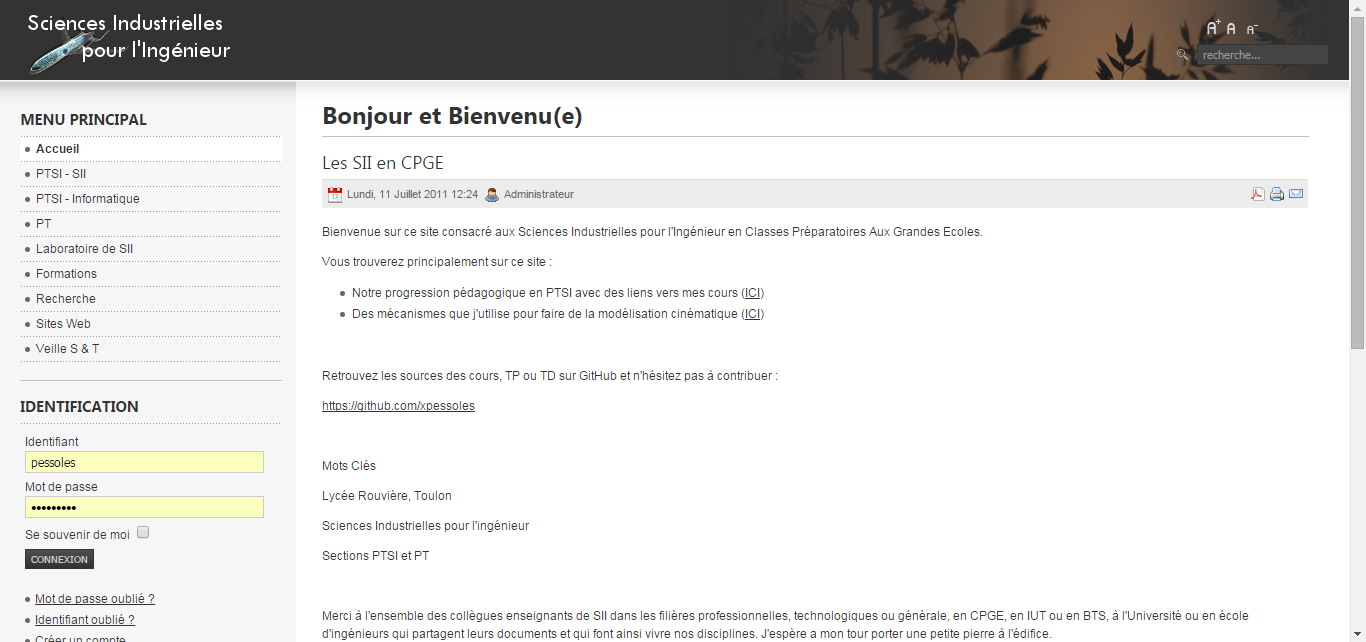
\includegraphics[height=2.5cm]{images/site_page}

\textit{Fichiers interprétés par un navigateur}
\end{center}
\end{minipage} \hfill
\begin{minipage}[c]{.33\linewidth}
\begin{center}
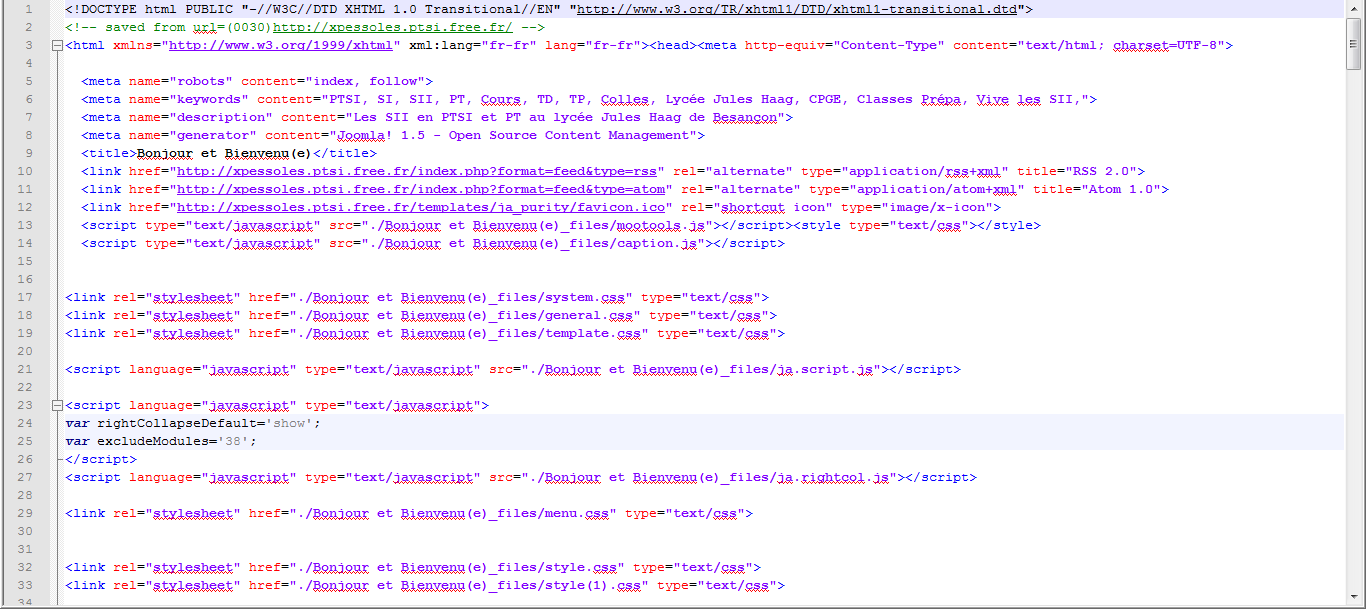
\includegraphics[height=2.5cm]{images/site_editeur}

\textit{Fichier interprété par un éditeur de texte}
\end{center}
\end{minipage} \hfill
\begin{minipage}[c]{.3\linewidth}
\begin{center}
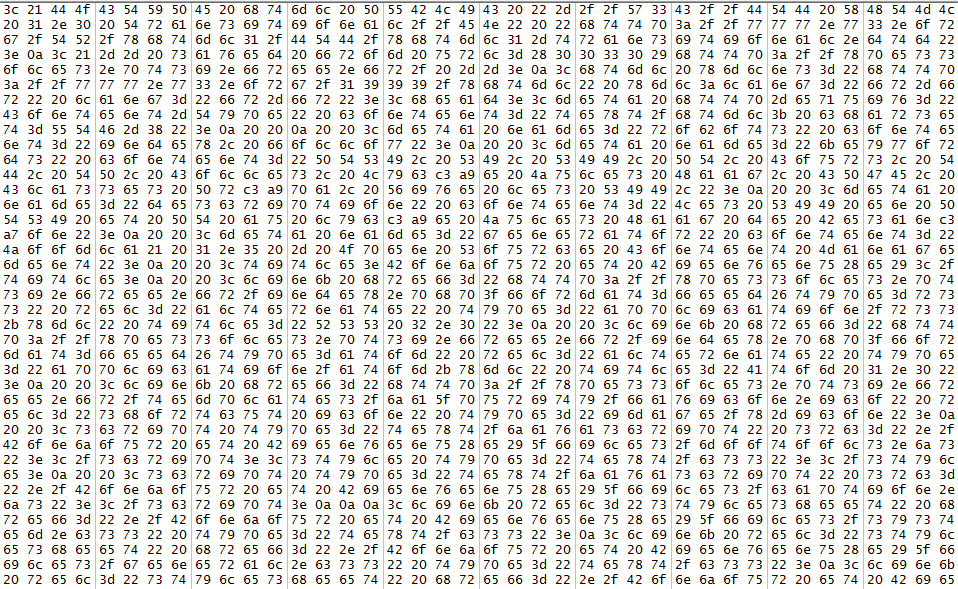
\includegraphics[height=2.5cm]{images/site_hexa}

\textit{Contenu du fichier (en hexadécimal)}
\end{center}
\end{minipage} 

\begin{savoir}
\textbf{Savoirs :}
\begin{itemize}
\item Manipuler des structures de données : chaînes de caractères (création, accès à un caractère, concaténation).
\item Gérer les fichiers : notion de chemin d'accès, lecture et écriture de données numériques ou de type de chaîne de caractère depuis ou vers un fichier.
\end{itemize}
\end{savoir}

\setlength{\parskip}{0ex plus 0.2ex minus 0ex}
 \renewcommand{\contentsname}{}
 \renewcommand{\baselinestretch}{1}

\tableofcontents

 \renewcommand{\baselinestretch}{1.2}
\setlength{\parskip}{2ex plus 0.5ex minus 0.2ex}

%\vspace{1cm}



%\newpage

\begin{minipage}[c]{.79\linewidth}
\section{Pourquoi utiliser des fichiers ?}

L'ordinateur sert à traiter de l'information qui peut entrer et sortir de différentes façons :
\begin{itemize}
\item le clavier, la souris et l'écran, pour l'interface utilisateur du programme ou le shell;
\item les fichiers, pour les supports mémoire;
\item les interfaces de communication (réseau, port USB, port série, etc.).
\end{itemize}

Le clavier et la souris ne permettent pas d'entrer une grosse masse d'information. De même l'écran montre une petite partie de l'information.
En revanche les fichiers permettent de décupler les possibilités de traitement d'information des programmes. Un roman de 200 pages contient environ 500 000 caractères, et donc tient en un fichier de 500 ko environ. 

Le réseau permet d'échanger des informations sous deux formes :
\begin{itemize}
\item sous forme de fichiers échangés, qui sont ensuite stockés sur le disque dur;
\item sous forme de flux de données. Ces données sont traitées par les cartes interfaces et mises à disposition des programmes par l'OS sous une forme proche des fichiers.
\end{itemize}
Il est donc intéressant de savoir lire et écrire sur les fichiers. 


\end{minipage} \hfill
\begin{minipage}[c]{.19\linewidth}
\begin{center}
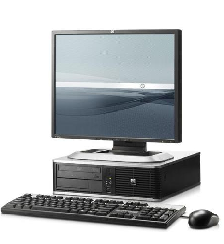
\includegraphics[width=.9\textwidth]{images/image1.png}
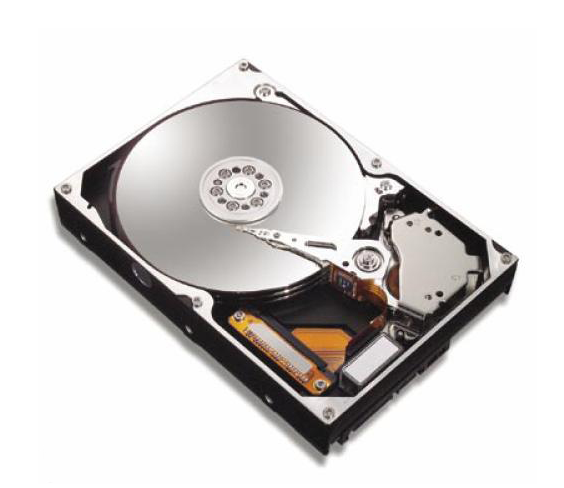
\includegraphics[width=.9\textwidth]{images/image2.png}
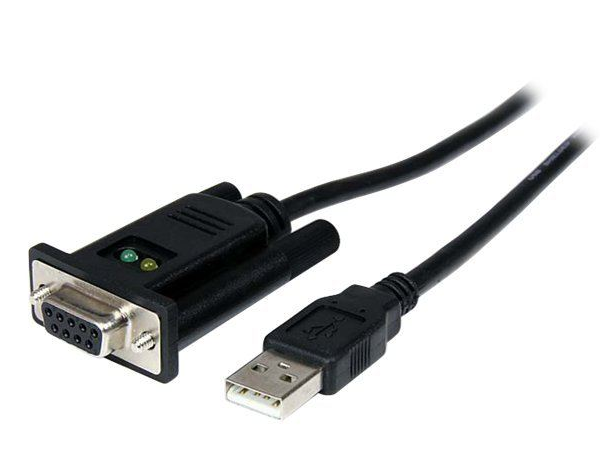
\includegraphics[width=.9\textwidth]{images/image3.png}
\end{center}
\end{minipage}






\subsection{Deux familles de fichiers}


\begin{minipage}[c]{.6\linewidth}

Les fichiers sont tous écrits en binaire. Il est néanmoins possible de les séparer en deux familles :
\begin{itemize}
\item les fichiers binaires qui nécessitent de connaître le format binaire d'écriture des données pour être lus;
\item les fichiers texte qui contiennent des caractères uniquement, et qui peuvent s'ouvrir sur un éditeur de texte.
\end{itemize}

\begin{exemple}

Les fichiers binaires :

\begin{itemize}
\item images et documents (bmp, png, jpg, pdf, doc, etc.);
\item son et vidéo (wav, mp3, mp4, etc.);
\item exécutables (.exe);
\item archives compressées (zip, 7z, gz).
\end{itemize}

Les fichiers texte :

\begin{itemize}
\item pages Web (html, css, etc.);
\item fichier journal (log), Script shell (bat);
\item images vectorielles (svg);
\item programmes Python ou Scilab (py, sce);
\item les fichiers de données texte (txt, data, etc.);
\item les fichiers texte formatés (xml).
\end{itemize}

Les fichiers texte compressés :
\begin{itemize}
\item les fichiers bureautique (odt, ods, docx, xlsx).
\end{itemize}
\end{exemple}

\end{minipage} \hfill
\begin{minipage}[c]{.32\linewidth}
\begin{center}
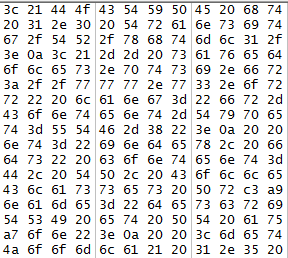
\includegraphics[width=.9\textwidth]{images/image4_2.png}

\vspace{1cm}
 
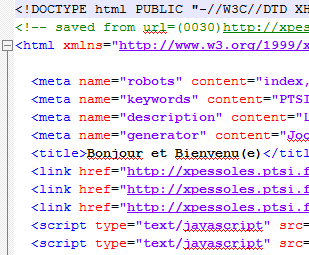
\includegraphics[width=.9\textwidth]{images/image5_2.png}
\end{center}
\end{minipage}





\subsection{Avantages et inconvénients}
\begin{center}
\begin{tabular}{|p{2.5cm}|p{6.5cm}|p{8cm}|}
\cline{2-3}
\multicolumn{1}{c|}{} & Fichiers binaire& Fichiers texte\\
 \hline
Avantages &  Moins volumineux & Interprétable par l'homme\\

		  & Indépendant des standards d'encodage des caractères dans les OS &Permet des d'échanges plus simples entre logiciels\\
		  & & Ne nécessite généralement pas de bibliothèques\\
\hline
Inconvénients & Moins facile à lire & Plus volumineux\\

			& Nécessite des bibliothèques pour les ouvrir &Dépendant du format d'encodage des caractères\\
			\hline
\end{tabular}
\end{center}

\subsection{Principe de manipulation d'un fichier}

Quel que soit le principe de manipulation du fichier il est toujours réalisé en trois opérations :
\begin{enumerate}
\item ouverture du fichier;
\item traitement du fichier;
\item fermeture du fichier.
\end{enumerate}


\section{Fichiers texte}


Un fichier texte brut ou fichier texte simple est un fichier dont le contenu représente uniquement une suite de caractères.
Bien qu'on l'oppose ici aux fichiers binaires il est lui aussi codé en binaire sur l'ordinateur. Cependant ce codage est basé sur une norme connue de tous les éditeurs de texte afin de traduire le fichier en une suite de caractères <<imprimables>>.
Les caractères considérés sont généralement les caractères imprimables, d'espaces et de retours à la ligne. La notion de fichier texte est subjective et dépend notamment des systèmes de codage de caractère considérés. Ainsi si l'encodage est inconnu, un texte brut quelconque est inexploitable.

 
Il existe de nombreux standards de codage, dont l'American Standard Code for Information Interchange   ASCII. Cette norme ancienne créée pour gérer des caractères latins non accentués (nécessaire pour écrire en anglais) est à la base de nombreux codages de caractères.

L'ASCII permet de coder 128 caractères numérotés de 0 à 127 et peut donc être codé sur 7 bits. Cependant, les ordinateurs travaillent la plupart du temps en multiple de 8 bits, le huitième bit est mis à 0. On a donc un octet par caractère.


\begin{center}
\footnotesize{\begin{tabular}{|ccc l||ccc||ccc||ccc|}
\hline 
\textbf{Décimal} & &\textbf{ASCII} & \textbf{Description} & \textbf{Décimal} && \textbf{ASCII} & \textbf{Décimal} && \textbf{ASCII} & \textbf{Décimal} && 
\textbf{ASCII}\\
\hline\hline
0 &00&NUL & Null 					&32&20&Space &64 &40& @	& 96  &60& ` \\
1 &01&SOH & Start of heading   		&33&21&! 	&65&41& A 	& 97 &61& a \\
2 &02&STX & Start of text       		&34&22&'' 	&66&42& B 	& 98 &62& b \\
3 &03&ETX & End of text       		&35&23&\# 	&67&43& C 	& 99 &63& c \\
4 &04&EOT & End of transmission 	&36&24&\$ 	&68&44& D 	& 100 &64& d \\
5 &05&ENQ & Enquiry 				&37&25&\% 	&69&45& E 	& 101&65& e \\
6 &06&ACQ & Acknowledge 			&38&26&\& 	&70&46& F 	& 102 &66& f \\
7 &07&BEL& Bell 					&39&27&' 	&71&47& G 	& 103 &67& g \\
8 &08&BS&Backsapce 				&40&28&(	&72&48& H 	& 104 &68& h \\
9 &09&TAB& horizontal tab 			&41&29&)	&73&49& I 	& 105 &69& i \\
10&0A&LF&New line feed, new line	&42&2A&*	&74&4A& J 	& 106 &6A& j \\
11&0B&VT& Vertical tab  			&43&2B&+	&75&4B& K 	& 107 &6B& k \\
12&0C&FF& NP form feed, new page 	&44&2C&`	&76&4C& L 	& 108 &6C& l \\  
13&0D&CR& Carriage return 			&45&2D&- 	&77&4D& M 	& 109 &6D& m \\
14&0E&SO& Shift out 				&46&2E&. 	&78&4E& N 	& 110 &6E& n \\
15&0F&SI& Shift in 				&47&2F&/ 	&79&4F& O 	& 111 &6F& o \\
16&10&DLE& Data link espace 		&48&30&0 	&80&50& P 	& 112 &70& p \\
17&11&DC1& Device control 1		&49&31&1 	&81&51& Q 	& 113 &71& q \\
18&12&DC2 &Device control 2		&50&32&2 	&82&52& R 	& 114 &72& r \\
19&13&DC3 &Device control 3		&51&33&3 	&83&53& S 	& 115 &73& s \\
20&14&DC4 &Device control 4		&52&34&4 	&84&54& T 	& 116 &74& t \\
21&15&NAK &Negative acknowledge	&53&35&5 	&85&55& U 	& 117 &75& u \\
22&16&SYN &Synchronous idle 		&54&36&6 	&86&56& V 	& 118 &76& v \\
23&17&ETB &End of trans. block 		&55&37&7 	&87&57& W 	& 119 &77& w \\
24&18&CAN &Cancel 				&56&38&8 	&88&58& X 	& 120 &78& x \\
25&19&EM &End of medium 			&57&39&9 	&89&59& Y 	& 121 &79& y \\
26&1A&SUB &Substitute 			&58&3A&: 	&90&5A& Z 	& 122 &7A& z \\
27&1B&ESC &Escape 				&59&3B&; 	&91&5B& [ 	& 123 &7B& \{ \\
28&1C&FS &File separator 			&60&3C&< 	&92&5C& $\backslash$ & 124 &7C& |\\
29&1D&GS &Group separator 		&61&3D&= 	&93&5D& ] 	& 125 &7D& \}\\
30&1E&RS &Record separator 		&62&3E&> 	&94&5E& $\hat{}$& 126 &7E& $\tilde{}$ \\
31&1F&US &Unit separator 			&63&3F&? 	&95&5F& \_ & 127 &7F& DEL\\
\hline
\end{tabular}}

\textit{Table des caractères ASCII}
\end{center}

L'absence d'accents rend cette norme insuffisante à elle seule,
ce qui rend nécessaire l'utilisation d'autres encodages: UTF-8 par exemple (UCS transformation format 8 bits) dans lequel chaque caractère est représenté par un index et son codage binaire donné par une table. Les 128 premiers caractères ont un codage identique en ASCII et UTF8 (par exemple <<A>> a pour code ASCII 65 et se code en UTF-8 par l'octet 65) puis d'autres caractères sont ajoutés.


\subsection{Lecture d'un fichier sous Python}

Les fichiers texte sont écrits (en binaire) de façon à respecter un des codes standards de caractères (utf8, iso-8859, ASCII...).
Ils peuvent s'ouvrir sur un éditeur de texte, ce qui permet de lire ou modifier le contenu beaucoup plus facilement qu'en binaire.


\newpage

\begin{exemple}

Exploitation d'un fichier de mesure sur l'axe Emericc: \textsf{Mesure\_axe\_Emericc.txt}.

\textbf{Objectif} : Lire les données (paramètres et mesures) et tracer les courbes.

\begin{itemize}
\item 12 lignes de paramètres;
\item 100 lignes de données;
\item 9 lignes de paramètres.
\end{itemize}

\begin{minipage}[c]{.36\linewidth}
\begin{center}
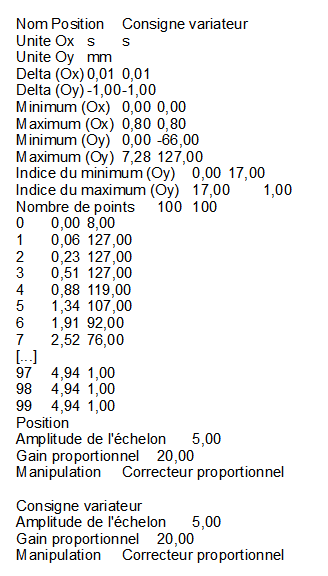
\includegraphics[width=.99\textwidth]{images/image11.png}
\end{center}
\end{minipage} \hfill
\begin{minipage}[c]{.6\linewidth}


\begin{py}
Lire la première ligne du fichier :
\begin{python}[H]
# Ouverture du fichier
f=open("Mesure_axe_Emericc.txt","r")
# lecture d'une ligne
ligne = f.readline()                  
# Affichage de la ligne
print(ligne)
# Fermeture du fichier
f.close()
\end{python}
Lecture rapide des lignes d'un fichier : 
\begin{python}[H]
# Ouverture du fichier
f=open("Mesure_axe_Emericc.txt","r")
for ligne in f :
    print(ligne)
f.close()
\end{python}
\end{py}

\end{minipage}




\begin{py}
Lecture des noms:
\begin{python}[H]
# Lecture d'un fichier texte ligne à ligne
# Ouverture fichier
f=open("TP_Fichiers/Mesure_axe_Emericc.txt","r")
ligne = f.readline()                  # lecture d'une ligne
# Affichage pour vérification
print(ligne)
ligne=ligne.rstrip("\n\r")            # suppression retour chariot
noms_grandeurs=ligne.split("\t")      # découpage aux tabulations
noms_grandeurs=noms_grandeurs[1:3]    # suppression de "noms"

\end{python}




Lecture du nombre de points:

\begin{python}[H]
for i in range(10):
    ligne = f.readline()  # saut de 10 lignes

ligne = f.readline()                  # lecture d'une ligne 
print(ligne)                    # affichage pour vérification
ligne=ligne.rstrip("\n\r")            # suppression retour chariot
ligne_nbpoints=ligne.split("\t")      # découpage aux tabulations
nb_points=int(ligne_nbpoints[1])      # conversion en entier
\end{python}

Lecture des données:

\begin{python}[H]

numero=[] ; position=[] ; consigne=[] # initialisation tableaux
for i in range(nb_points):
    ligne = f.readline()              # lecture d'une ligne 
    ligne=ligne.rstrip("\n\r")        # suppression retour chariot
    ligne=ligne.replace(",",".")      # changement , en .
    ligne_data=ligne.split("\t")      # découpage aux tabulations
    numero.append(int(ligne_data[0]))
    position.append(float(ligne_data[1]))    # Ajout aux tableaux
    consigne.append(float(ligne_data[2]))
\end{python}


Fermeture du fichier et Tracé de la courbe

\begin{python}[H]
f.close()        # Fermeture fichier
plot(position)   # Tracé de la courbe de position
\end{python}
\end{py}

\begin{center}
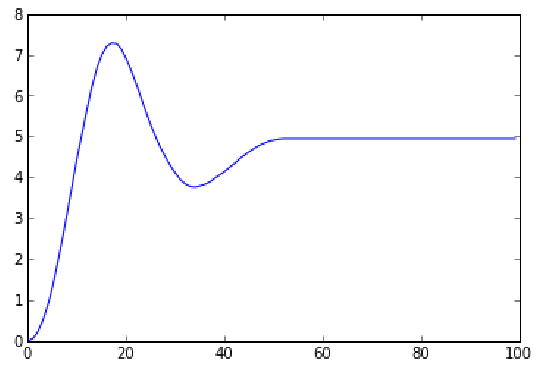
\includegraphics[width=.5\textwidth]{images/image9.png}
\end{center}


\end{exemple}


\subsection{Lecture d'un fichier sous Scilab}

De la même façon que Python, Scilab permet de lire des fichiers. La syntaxe est proche :

\begin{sci}
\begin{scilab}[H]
// Ouverture du fichier et lecture ligne a ligne
fic=mopen("Mesure_axe_Emericc.txt","r");
ligne=mgetl(fic,1)
// Decoupage a la tabulation = caractere ascii 9
noms_grandeurs=strsplit(ligne,ascii(9))
noms_grandeurs=noms_grandeurs(2:3)
for i=1:10
    ligne = mgetl(fic,1);
end

ligne = mgetl(fic,1)
ligne_nbpoints=strsplit(ligne,ascii(9))
nb_points=int(ligne_nbpoints(2))
nb_points=msscanf(ligne_nbpoints(2),"%i")
\end{scilab}



Lecture des données et affichage de la courbe.


\begin{scilab}[H]
numero=[];position=[];consigne=[];
for i=1:nb_points
    ligne = mgetl(fic,1);
    ligne = strsubst(ligne,",",".");
    [n,numero(i),position(i),consigne(i)]=msscanf(ligne,"%d\t%f\t%f");
end
mclose(fic);                    // Fermeture du fichier
plot(position)
\end{scilab}
\end{sci}




\begin{minipage}[c]{.69\linewidth}

\subsection{Cas des données formatées}
Le tableau de données est <<~formaté~>>, c'est-à-dire qu'il présente une structure identique à chaque ligne.

Python possède des outils de lecture automatique de ce type de tableau : numpy.loadtxt()

\begin{py}
\begin{python}[H]
a=loadtxt("Fichier.txt",
		dtype={
			'names': ('numero', 'position', 'consigne'),
			'formats': ('i2', 'f4', 'f4')},
		delimiter='\t')
\end{python}
\end{py}

\end{minipage} \hfill
\begin{minipage}[c]{.29\linewidth}
\begin{tabular}{ccc}
\hline
Int	&float	&	float\\
\hline
0	&0,00		&8,00\\
1	&0,06	&	127,00\\
2&	0,23	&	127,00\\
3&	0,51	&	127,00\\
4&	0,88	&	119,00\\
5&	1,34	&	107,00\\
6&	1,91	&	92,00\\
7&	2,52	&	76,00\\
... &...  &...  \\
97&	4,94	&	1,00\\
98&	4,94	&	1,00\\
99&	4,94	&	1,00\\
\hline
\end{tabular}


\end{minipage}



Pour récupérer les données :
\begin{py}
\begin{python}[H]
a['numero']			#liste de valeurs de la colonne N
a['numero'][10]			#11ème élément
\end{python}
\end{py}


\begin{figure}[H]
\begin{minipage}[c]{.59\linewidth}

\begin{py}
\begin{python}[H]
a,b=loadtxt("Fichier.txt",
		usecols = (0,2),
		dtype={
			'names': ('numero', 'consigne'),
			'formats': ('i2', 'f4')},
		delimiter='\t',
		unpack=True)
\end{python}
\end{py}

\end{minipage} \hfill
\begin{minipage}[c]{.39\linewidth}
\begin{itemize}
\item usecols : colonnes à utiliser dans le fichier
\item dtype : type de données à lire
\item Names : nom
\item format : entier sur 2o, flottant sur 4o, strings...
\item délimiter : séparateur des données
\item unpack : permet de séparer les colonnes → a,b=...
\end{itemize}
\end{minipage}
\end{figure}


\begin{figure}[H]
\begin{minipage}[c]{.49\linewidth}

\begin{py}
\begin{python}[H]
plot(a['numero'],a['position'],'b',
		a['numero'],a['consigne']/10,'r')
\end{python}
\end{py}

\end{minipage} \hfill
\begin{minipage}[c]{.49\linewidth}
\begin{center}
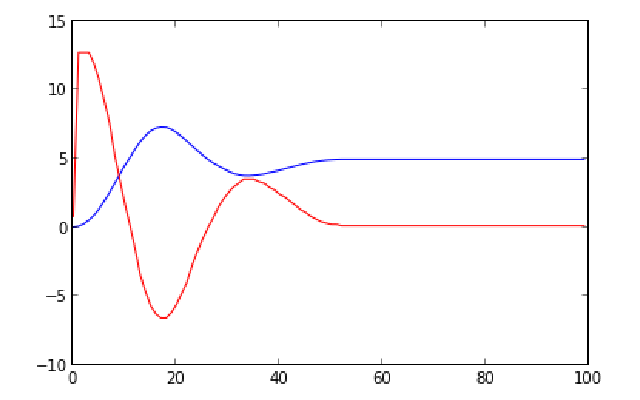
\includegraphics[width=.99\textwidth]{images/image10.png}
\end{center}
\end{minipage}
\end{figure}

\subsection{Lecture d'un fichier texte formaté sous Scilab}

\begin{figure}[H]
\begin{minipage}[c]{.49\linewidth}


De la même façon que Python, Scilab permet de lire des fichiers formatés.

La synthaxe est proche (en plus simple quand même...).

\end{minipage} \hfill
\begin{minipage}[c]{.49\linewidth}
\begin{sci}
\begin{scilab}[H]
// Lecture de donnees formatees
fic=mopen("Mesure_axe_Emericc_formate.txt","r");
T=mfscanf(-1,fic,'%d\t%f\t%f')  
plot(T(:,1),[T(:,2),T(:,3)/10])
mclose(fic);               // Fermeture du fichier
\end{scilab}
\end{sci}
\end{minipage}
\end{figure}




\subsection{Écriture d'un fichier texte sous python}
L'écriture d'un fichier texte est très simple sous python:
\begin{py}
\begin{python}[H]
# Écriture d'un fichier texte ligne à ligne
f=open("TP_Fichiers/monFichier.txt","w")  # Ouverture du fichier
f.write("La température est froide l'hiver.\n")
f.write("Il fait {:f} degrés.".format(10))
f.close()        # Fermeture du fichier
\end{python}
\end{py}

Et pour un fichier formaté :
\begin{py}
\begin{python}[H]
# Écriture d'un fichier formaté
f=open("TP/monFichier.txt","w")  # ouverture fichier
x=linspace(-20,20,100)
y=sin(x)/x
for i in range(0,len(x)):
    f.write(str(x[i])+"\t"+str(y[i])
f.close()        # Fermeture du fichier
\end{python}
\end{py}

\subsection{Écriture d'un fichier texte sous Scilab}
L'écriture d'un fichier texte, formaté ou pas, est très simple :
\begin{sci}
\begin{scilab}[H]
// Ecriture de donnees formatees ou non...
fic=mopen("monFichier.txt","w");
mfprintf(fic,"Voici mon fichier de point\n")
mfprintf(fic,"Nombre de points : %d\n",100)
x=-20:40/99:20;
y=sin(x)./x;
mfprintf(fic,'%d\t%f\t%f\n',[1:100]',x',y')  
mclose(fic); // Fermeture du fichier
\end{scilab}
\end{sci}


\section{Fichiers binaires}

\subsection{Analyse d'un fichier binaire : BMP}

\begin{minipage}[c]{.53\linewidth}

On peut ouvrir un fichier binaire avec un éditeur héxadécimal.

Les deux premiers caractères de cette exemple "42" représentent en hexadécimal le codage sur les 8 bits correspondants (celui-ci apparait en bas de la fenêtre quand on se place sur le "42").

Un fichier BMP est un format très simple pour mémoriser les images:
\begin{itemize}
\item signature (BM, BA, CI, …);
\item taille du fichier (4o);
\item champ réservé (4o);
\item offset de début données (4o);
\item taille de l'entête (4o);
\item largeur de l'image (4o);
\item hauteur de l'image (4o);
\item nombre de plans (2o);
\item profondeur : 1 à 32 (2o);
\item type compression (4o);
\item etc.
\end{itemize}


Les couleurs commencent à l'octet 122=0x7A (octet en jaune) :
\begin{itemize}
\item blanc (ff ff ff);
\item blanc (ff ff ff);
\item blanc (ff ff ff);
\item blanc (ff ff ff);
\item gris clair (e9 ec ef);
\item gris (ce cc c4);
\item gris foncé (a0 97 7c)...
\end{itemize}
\begin{center}

\includegraphics[width=.5\textwidth]{images/image8.png}
\end{center}
\end{minipage} \hfill
\begin{minipage}[c]{.25\linewidth}
\begin{center}

\includegraphics[width=.5\textwidth]{images/image6.png}
\end{center}
\begin{center}
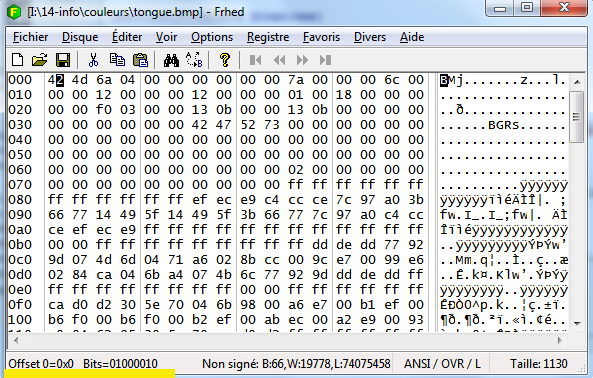
\includegraphics[width=.99\textwidth]{images/image12.png}
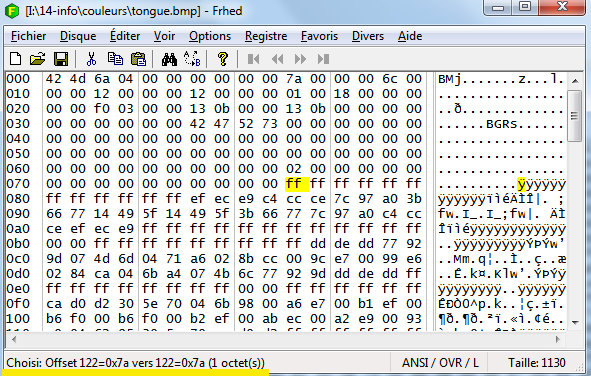
\includegraphics[width=.99\textwidth]{images/image13.png}
\textit{Ouverture d'un fichier binaire avec un éditeur hexadécimal}
\end{center}
\end{minipage}







\subsection{Ouvrir des fichiers binaires}
Les formats étant généralement assez complexes et variés, les fichiers binaires sont ouverts via des \textbf{librairies}. Ces librairies proposent des commandes toutes prêtes. Par exemple pour les images :
\begin{itemize}
\item Python : librairie PIL (Python Imaging Library);
\item Scilab inclut des commandes pour les images.
\end{itemize}

On code très rarement les commandes permettant d'ouvrir les fichiers binaires.
Pour lire tout de même un fichier binaire on utilise la fonction \textsf{open}, disponible sans aucune bibliothèque. Elle prend en paramètre :
\begin{itemize}
\item le chemin (absolu ou relatif) menant au fichier à ouvrir;
\item le mode d'ouverture.
\end{itemize}

Le mode est donné sous la forme d'une chaîne de caractères. Voici les principaux modes :
\begin{itemize}
\item 'r' : ouverture en lecture (Read);
\item 'w' : ouverture en écriture (Write). Le contenu du fichier est écrasé. Si le fichier n'existe pas, il est créé,
\item 'a' : ouverture en écriture en mode ajout (Append). On écrit à la fin du fichier sans écraser l'ancien contenu du fichier. Si le fichier n'existe pas, il est créé.
\end{itemize}

On peut ajouter à tous ces modes le signe b pour ouvrir le fichier en mode binaire.

La fonction open crée un objet de la classe \textsf{TextIoWrapper}. Par la suite, nous allons utiliser des méthodes de cette classe pour interagir avec le fichier.

\begin{minipage}[c]{.49\linewidth}

\begin{py}
\begin{python}[H]
# Lecture d'un fichier binaire
f = open("tongue.bmp", "rb")

while True:
	bytes = f.read(1) # lecture d'un octet
	if bytes == "":
	    break;
	# Affichage de l'octet lu en hexadécimal :
	print "%02X " % ord(bytes[0]),

f.close()
\end{python}
\end{py}



\end{minipage} \hfill
\begin{minipage}[c]{.49\linewidth}
3 étapes:
\begin{enumerate}
\item Ouverture du fichier “tongue.bmp”, en lecture mode binaire (“rb”).
\item Boucle sur chaque octet pour lire et afficher. La méthode read renvoie le contenu du fichier, que l'on capture dans bytes.
\item Fermeture du fichier: n'oubliez pas de fermer un fichier après l'avoir ouvert. Si d'autres applications, ou d'autres morceaux de votre propre code, souhaitent accéder à ce fichier, ils ne pourront pas car le fichier sera déjà ouvert. C'est surtout vrai en écriture, mais prenez de bonnes habitudes. La méthode à utiliser est \textsf{close}.
\end{enumerate} 
\end{minipage}


\subsection{Écrire dans des fichiers en binaire}


\begin{minipage}[c]{.39\linewidth}

\begin{py}
\begin{python}[H]
# Écriture d'un fichier binaire
f=open("TP/monFichier.bin","wb")
f.write("Du texte")
f.write(int8(83))
f.write(int8(76))
f.write(float32(2.3))
f.close()
\end{python}
\end{py}

\end{minipage} \hfill
\begin{minipage}[c]{.59\linewidth}
3 étapes:
\begin{enumerate}
\item Il faut ouvrir le fichier avant tout. Ouverture du fichier “monFichier.bin”, en écriture mode binaire (“wb”).
\item Écriture d'octets (caractères, nombres entiers ou flottants): On utilise la méthode write. Deux modes sont possibles: le mode w ou le mode a. Le premier écrase le contenu éventuel du fichier, alors que le second ajoute ce que l'on écrit à la fin du fichier. Ces deux modes créent le fichier s'il n'existe pas.
\item Fermeture du fichier. 
\end{enumerate}
\end{minipage}




\section{Enregistrer un objet dans un fichier: Module Pickle}

Dans Python comme dans beaucoup de langages de haut niveau, on peut enregistrer les objets dans un fichier. 
Lorsque l'objectif est de sauver des objets python pour les récupérer plus tard sous python, il est pratique d'utiliser Pickle.

Alors que les fonctions utilisées dans ce cours ne nécessitaient pas l'importation de bibliothèque, il faut penser ici à importer Pickle.

Soit v une variable quelconque,

\begin{minipage}[t]{.49\linewidth}

Sauvegarde :


\begin{py}
\begin{python}[H]
import pickle
fic=open("nao.pick","wb")
pickle.dump(v,fic)
fic.close()
\end{python}
\end{py}

On utilise la méthode dump pour enregistrer l'objet.

Une fois ce code exécuté un fichier nao.pick aura été créé avec les données correspondantes à l'intérieur.

Pour stocker plusieurs variables, il suffit d'appeler plusieurs fois la fonction pickle.dump() pour chaque variable.

\end{minipage} \hfill
\begin{minipage}[t]{.49\linewidth}

Lecture :	

\begin{py}
\begin{python}[H]
import pickle
fic=open("nao.pick","rb")
v=pickle.load(fic)
fic.close()
\end{python}
\end{py}



Pour recharger ces variables, il faut appeler autant de fois la fonction pickle.load(). Les variables sont restituées dans le même ordre.

\end{minipage}


\begin{thebibliography}{2}
\bibitem{upsti}{Marc Derumeaux et Damien Iceta, \textit{Les fichiers. Apprendre à lire et à écrire}, UPSTI.}
%\bibitem{wack}{Wack et Al., \textit{L'informatique pour tous en classes préparatoires aux grandes écoles}, Editions Eyrolles.}
\end{thebibliography}
\end{document}


